%===============================================================================
% LaTeX sjabloon voor de bachelorproef toegepaste informatica aan HOGENT
% Meer info op https://github.com/HoGentTIN/bachproef-latex-sjabloon
%===============================================================================

\documentclass{bachproef-tin}

\usepackage{hogent-thesis-titlepage} % Titelpagina conform aan HOGENT huisstijl
\usepackage{lipsum}
\usepackage{float}



%%---------- Documenteigenschappen ---------------------------------------------
% TODO: Vul dit aan met je eigen info:

% De titel van het rapport/bachelorproef
\title{Geautomatiseerd parsen van systeem logs}

% Je eigen naam
\author{Marbod Naassens}

% De naam van je promotor (lector van de opleiding)
\promotor{Stijn Lievens}

% De naam van je co-promotor. Als je promotor ook je opdrachtgever is en je
% dus ook inhoudelijk begeleidt (en enkel dan!), mag je dit leeg laten.
\copromotor{Geert De Paep}

% Indien je bachelorproef in opdracht van/in samenwerking met een bedrijf of
% externe organisatie geschreven is, geef je hier de naam. Zoniet laat je dit
% zoals het is.
\instelling{---}

% Academiejaar
\academiejaar{2020-2021}

% Examenperiode
%  - 1e semester = 1e examenperiode => 1
%  - 2e semester = 2e examenperiode => 2
%  - tweede zit  = 3e examenperiode => 3
\examenperiode{2}

%===============================================================================
% Inhoud document
%===============================================================================

\begin{document}

%---------- Taalselectie -------------------------------------------------------
% Als je je bachelorproef in het Engels schrijft, haal dan onderstaande regel
% uit commentaar. Let op: de tekst op de voorkaft blijft in het Nederlands, en
% dat is ook de bedoeling!

%\selectlanguage{english}

%---------- Titelblad ----------------------------------------------------------
\inserttitlepage

%---------- Samenvatting, voorwoord --------------------------------------------
\usechapterimagefalse
%%=============================================================================
%% Voorwoord
%%=============================================================================

\chapter*{\IfLanguageName{dutch}{Woord vooraf}{Preface}}
\label{ch:voorwoord}

%% TODO:
%% Het voorwoord is het enige deel van de bachelorproef waar je vanuit je
%% eigen standpunt (``ik-vorm'') mag schrijven. Je kan hier bv. motiveren
%% waarom jij het onderwerp wil bespreken.
%% Vergeet ook niet te bedanken wie je geholpen/gesteund/... heeft

Dit onderwerp was iets wat mij persoonlijk aansprak omdat ik zelf reeds in aanraking ben gekomen met log bestanden. Als er problemen zijn binnen een programma dat ik gebruik dan ga ik hiernaar kijken om er wijzer uit te worden of om deze mee te geven aan de klantenservice. Hierbij geraak ik zelf niet altijd uit aan de betekenis van de logs en zelfs de klantenservice van grote bedrijven weten hier niet altijd raad mee. Daarom leek het onderzoeken van algoritmes die deze bestanden leesbaarder maakten een leuk bachelorproef onderwerp.\\

Persoonlijk wist ik zelf niet veel over de wereld van log parsers en daarom vond ik dit ook een goede leerervaring. Ik heb veel bijgeleerd bij het onderzoek, maar omdat dit veel verschillende papers inhield en deze niet altijd even duidelijk waren voor iemand die losstaat van de logging wereld was dit wel niet altijd even makkelijk. Het was wel een leuke ervaring en ik hoop dat deze bachelorproef een meerwaarde kan vormen voor mijn promotor en co-promotor zodat ze dit in hun toekomstig werk kunnen benutten.\\

Deze bachelorproef zou nooit tot stand gekomen zijn zonder hulp van verschillende personen. Deze wil ik hieronder bedanken:
\begin{itemize}
    \item Christina Christiaens: Eerst en vooral wil ik mijn vriendin bedanken voor al haar steun en geduld tijdens de maanden van mijn bachelorproef en voor het nalezen van mijn bachelorproef.
    \item Stijn Lievens: Mijn promotor wil ik bedanken voor de consistente en duidelijke opvolging. Ik kon voor al mijn vragen bij hem terecht en hij kon mij altijd goed verder helpen, ook wil ik hem bedanken voor het tussentijds evalueren en nalezen van mijn bachelorproef. 
    \item Geert De Paep: Mijn co-promotor wil ik bedanken voor het nalezen van mijn voorstel, het geven van goede raad en de hulp bij het integreren van nieuwe datasets in mijn onderzoek.
    \item Simon De Wilde: Ik wil mijn medestudent Simon bedanken voor het helpen bij problemen met de bachelorproef en voor zijn geduld bij mijn vragen.
    \item Ziggy Moens: Ik wil mijn medestudent Ziggy bedanken voor het nalezen van mijn voorstel, het nalezen van de integratie bij de Stand van Zaken, het geven van raad en het bijstaan bij problemen.
\end{itemize}

%%=============================================================================
%% Samenvatting
%%=============================================================================

% TODO: De "abstract" of samenvatting is een kernachtige (~ 1 blz. voor een
% thesis) synthese van het document.
%
% Deze aspecten moeten zeker aan bod komen:
% - Context: waarom is dit werk belangrijk?
% - Nood: waarom moest dit onderzocht worden?
% - Taak: wat heb je precies gedaan?
% - Object: wat staat in dit document geschreven?
% - Resultaat: wat was het resultaat?
% - Conclusie: wat is/zijn de belangrijkste conclusie(s)?
% - Perspectief: blijven er nog vragen open die in de toekomst nog kunnen
%    onderzocht worden? Wat is een mogelijk vervolg voor jouw onderzoek?
%
% LET OP! Een samenvatting is GEEN voorwoord!

%%---------- Nederlandse samenvatting -----------------------------------------
%
% TODO: Als je je bachelorproef in het Engels schrijft, moet je eerst een
% Nederlandse samenvatting invoegen. Haal daarvoor onderstaande code uit
% commentaar.
% Wie zijn bachelorproef in het Nederlands schrijft, kan dit negeren, de inhoud
% wordt niet in het document ingevoegd.

\IfLanguageName{english}{%
\selectlanguage{dutch}
\chapter*{Samenvatting}
\lipsum[1-4]
\selectlanguage{english}
}{}

%%---------- Samenvatting -----------------------------------------------------
% De samenvatting in de hoofdtaal van het document

\chapter*{\IfLanguageName{dutch}{Samenvatting}{Abstract}}

\lipsum[1-4]


%---------- Inhoudstafel -------------------------------------------------------
\pagestyle{empty} % Geen hoofding
\tableofcontents  % Voeg de inhoudstafel toe
\cleardoublepage  % Zorg dat volgende hoofstuk op een oneven pagina begint
\pagestyle{fancy} % Zet hoofding opnieuw aan

%---------- Lijst figuren, afkortingen, ... ------------------------------------

% Indien gewenst kan je hier een lijst van figuren/tabellen opgeven. Geef in
% dat geval je figuren/tabellen altijd een korte beschrijving:
%
%  \caption[korte beschrijving]{uitgebreide beschrijving}
%
% De korte beschrijving wordt gebruikt voor deze lijst, de uitgebreide staat bij
% de figuur of tabel zelf.

\listoffigures
\listoftables

% Als je een lijst van afkortingen of termen wil toevoegen, dan hoort die
% hier thuis. Gebruik bijvoorbeeld de ``glossaries'' package.
% https://www.overleaf.com/learn/latex/Glossaries

%---------- Kern ---------------------------------------------------------------

% De eerste hoofdstukken van een bachelorproef zijn meestal een inleiding op
% het onderwerp, literatuurstudie en verantwoording methodologie.
% Aarzel niet om een meer beschrijvende titel aan deze hoofstukken te geven of
% om bijvoorbeeld de inleiding en/of stand van zaken over meerdere hoofdstukken
% te verspreiden!

%%=============================================================================
%% Inleiding
%%=============================================================================

\chapter{\IfLanguageName{dutch}{Inleiding}{Introduction}}
\label{ch:inleiding}

%%De inleiding moet de lezer net genoeg informatie verschaffen om het onderwerp te begrijpen en in te zien waarom de onderzoeksvraag de moeite waard is om te onderzoeken. In de inleiding ga je literatuurverwijzingen beperken, zodat de tekst vlot leesbaar blijft. Je kan de inleiding verder onderverdelen in secties als dit de tekst verduidelijkt. Zaken die aan bod kunnen komen in de inleiding~\autocite{Pollefliet2011}:

%%\begin{itemize}
  %%\item context, achtergrond
  %%\item afbakenen van het onderwerp
  %%\item verantwoording van het onderwerp, methodologie
  %%\item probleemstelling
  %%\item onderzoeksdoelstelling
  %%\item onderzoeksvraag
  %%\item \ldots
%%\end{itemize}

Het geautomatiseerd parsen van systeem logs klinkt als een complexe casus en uit de titel kan men het probleemdomein niet onmiddelijk afleiden. Om deze titel en aldus het onderwerp beter te begrijpen moet men ten eerste begrijpen binnen welke context het parsen van systeem logs plaatsvindt. Voordat het domein zal toegelicht worden is het handig om eerst nog toe te lichten wat systeem logs specifiek zijn. Hierover geeft de eerste sectie wat meer informatie. Een tweede onderwerp, dat cruciaal is binnen dit onderzoek, is wat het parsen van logs specifiek inhoudt. Hierop wordt dieper ingegaan in de tweede sectie. Een belangrijk begrip bij het parsen van logs is `reguliere expressies`, reguliere expressies worden binnen applicatieontwikkeling veel benut en zijn ook een zeer belangrijk onderdeel bij het parsen van logs. De derde sectie zal dit begrip verder bespreken. In de laatste sectie wordt er dieper ingegaan op het specifieke domein waarop toegespitst wordt binnen deze bachelorproef. Deze bachelorproef beperkt zich tot systeem logs alsook zal het parsen van de logfiles als voorbereiding op anomaliedetectie toegepast worden. 

\section{Wat is een log?}

Een systeem log is een log file gelinkt aan een bepaald systeem (zoals bv. Windows, Linux, etc.). Een log file is een primaire data bron voor observaties. Het is een datafile gegenereerd door een computer die informatie bevat over gebruikpatronen, activiteiten en operaties die plaatsvinden binnen een operating system, een applicatie, een server of een apparaat. Log files worden gegenereerd wanneer specifieke handelingen gebeuren over het netwerk of binnen de applicatie. Organisaties binnen de IT sector gebruiken logfiles om het gebruik en de activiteiten van hun gebruikers te analyseren en ook om het gedrag van de applicatie vast te leggen voor eventuele verbeteringen of fouten te detecteren. De hoofdreden waarom log files bestaan is omdat ontwikkelaars van software en hardware het makkelijker vinden om via tekstuele data de werking van het systeem te volgen en vast te leggen. Voor elk domein binnen IT zijn er verschillende logs, voor security, servers, applicaties, etc. Daarbovenop zijn de logs ook nogmaals verschillend van bedrijf tot bedrijf (Google, Apple, Microsoft, etc.).

\section{Log Parsing}

Log parsing is een methode die wordt toegepast bij het analyseren van log files. Voordat men een logfile kan analyseren moet men eerst de logfile kunnen opdelen in verschillende delen en deze delen van een label voorzien. Dit is waarvoor men parsers gebruikt. Log parsing is vooral belangrijk om een logfile goed te kunnen analyseren want door logparsing toe te passen kan men specifieke data uit de logs, zoals timestamp, hostname, service name, etc., makkelijk afleiden. Log parsing kan op verschillende manieren gebeuren. Hieronder worden enkele methodologieën, i.e.\ manieren om loglijnen op te delen in stukken die makkelijker te analysteren zijn, die van belang zijn binnen het onderzoek van deze bachelorproef opgelijst en verder toegelicht:
\begin{itemize}
    \item Regex, hierbij worden reguliere expressies toegepast om alle velden van een systeem log te ontleden. Reguliere expressies zijn een opeenvolging van symbolen en karakters die een string of patroon waarnaar gezocht wordt binnen een tekst voorstellen.
    \item Grok, combineert meerdere tekstpatronen naar iets dat overeenkomt met de logs. Dit om logs op te delen in verschillende delen zodat logs mooi gestructureerd worden en er queries op kunnen uitgevoerd worden.
    \item Parse operator, custom manieren om logs op te delen. Gebruikt als Grok of Regex geen goeie structuur opleveren.
\end{itemize}
Log parsing methodes worden toegepast op verschillende manieren met verschillende strategieën. Deze strategieën ondersteunen de toepassing van de methodologieën. Hieronder worden de verschillende strategieën binnen het onderzoek van deze bachelorproef toegelicht:
\begin{itemize}
    \item Frequent pattern mining: Deze techniek is gebaseerd op frequente patronen die vaak voorkomen in bepaalde datasets.
    Zo kunnen bijvoorbeeld events in een log gezien worden als constante tokens die vaak voorkomen. De procedure die hiermee gepaard gaat is als volgt:\\
    \begin{enumerate}
        \item De log data meerdere keren overlopen.
        \item Opbouwen van frequente items en patronen bij elke iteratie.
        \item Groeperen van log messages in verschillende clusters.
        \item Het extraharen van event templates bij elke cluster. 
    \end{enumerate} 
    \item Clustering: Bepaalde loglijnen kunnen voldoen aan eenzelfde opbouw of `template`. Deze loglijnen hebben een gelijkaardige vorm. Uit log files kan men meerdere vormen halen en deze definiëren in een beperkt aantal clusters. Elke loglijn wordt onderzocht en als deze voldoet aan het template van één van deze clusters dan wordt de loglijn toegevoegd aan deze cluster. Zo niet, dan wordt op basis van de loglijn een nieuwe cluster aangemaakt.
    \item Heuristieken: Loglijnen hebben unieke karakteristieken waardoor men heuristieken kan toepassen binnen de logparsing. Dit kan op verschillende manieren:\\
    \begin{enumerate}
        \item Het verdelen in meerdere groepen van loglijnen op basis van het aantal voorkomens van constante en variabele tokens.
        \item Door te verdelen op basis van de lengte van de log messages, de token positie, i.e.\ waar in de log de message plaatsvindt, en mapping relaties.
        \item Met een diepte-gelimiteerde boom de relaties vastleggen en partitioneren.
    \end{enumerate}
\end{itemize}
Andere strategieën bestaan nog maar worden niet verder toegelicht in het onderzoek van deze bachelorproef.

\section{Reguliere Expressie}
Binnen de log parsing methodes die zullen behandeld worden in dit onderzoek zullen reguliere expressies regelmatig aangehaald worden. Dit is omdat reguliere expressies één van de makkelijkste en meest performante manieren zijn om data op te halen uit tekst bestanden. Een reguliere expressie is een manier om patronen te beschrijven waardoor een programma verschillende soorten tekst kan herkennen. Reguliere expressies worden vooral gebruikt om bepaalde stukken uit teksten te filteren. Voorbeelden hiervan zijn: Achterhalen of een bepaalde tekst een email adres bevat, kijken of een paswoord de juiste tekens bevat, etc.. Reguliere expressies hebben een universele syntax waardoor deze niet afhankelijk zijn van programma of software. Hierdoor wordt natuurlijk direct duidelijk waarom reguliere expressies zo krachtig zijn binnen het parsen van logs. Ze zijn software onafhankelijk en stellen ons in staat om efficiënt logs te overlopen en te zien of ze aan een bepaalde syntax voldoen. Zo worden reguliere expressies gebruikt binnen Drain om al een eerste filtering door de log messages uit te voeren. Hieronder wordt een voorbeeld gegeven van een reguliere expressie voor het vinden van een email.
\begin{verbatim}
    ^[a-zA-Z\.]+@([a-zA-Z]+\.)+[a-zA-Z]{2,4}$
\end{verbatim}

Dit voorbeeld ziet er complex uit maar de betekenis is makkelijk te achterhalen. Er wordt begonnen met een \verb!^! dit geeft het begin van de string aan. Hierna volgt \verb![a-zA-Z\.]!, hierbij wordt aangegeven dat het begint met een reeks letters, die beide grote en kleine letters kunnen zijn van \(a\) tot \(z\), en deze letterreeks wordt dan gevolgd door een punt, dit wordt aangegeven door de \verb!\.!. De schuine streep is nodig voor aan te geven dat het om een speciaal karakter gaat. Na het plusteken volgt de \verb!@! om aan te geven dat er een \verb!@! moet staan, dit is logisch voor een email adres. Hierna wordt weer aangegeven dat er een letter reeks met punten mogelijk is, die dan finaal gevolgd wordt door een letter reeks bestaande uit minimum 2 en maximum 4 letters, hiervoor wordt de \(\{2,4\}\) gebruikt.\\

Nog een veel voorkomende reguliere expressie binnen deze bachelorproef zal de reguliere expressie voor een IPv4 of IPv6 adres zijn. Hieronder worden respectievelijk reguliere expressies voor beide gegeven.
\begin{verbatim}
    ^[[0-9]{1,4}\.]{3}+[0-9]{1,4}$
\end{verbatim}
\begin{verbatim}
    ^[[0-9a-z]{4}\:]{7}+[0-9a-z]{4}$
\end{verbatim}
Hier zien we dat er bij IPv4 begonnen wordt met een combinatie van vier cijfers van nul tot negen, aangegeven door \([0-9]\{1,4\}\), gevolgd door een punt. Deze soort sequentie komt exact drie keer voor en dan nog een laatste keer zonder punt. De reguliere expressie voor het IPv6 patroon is gelijk lopend maar hierbij zien we dat de sequentie zeven keer plaatsvindt met een dubbele punt (\(:\)). Hierbij is het ook duidelijk dat het over een hexadecimale sequentie door \([0-9a-z]\). Dit geeft aan dat het karakter uit een getal van nul tot negen of een letter van a tot z kan bestaan.

\section{Anomalie Detectie}

Anomaliedetectie is een moeilijk begrip omdat het een breed onderwerp is. In het algemeen is anomaliedetectie het vinden van patronen binnen de data van een bepaald systeem of een bepaalde applicatie die niet voldoen aan het verwachte gedrag. Deze patronen worden anomalieën genoemd \autocite{chandola2009anomaly}. Men doet aan anomaliedetectie om applicaties en systemen zo performant en betrouwbaar mogelijk te houden. Voorbeelden hiervan zijn fraude detectie binnen bank applicaties (credit cards, etc.), indringers detectie binnen cybersecurity en zelfs binnen militaire surveillance om vijanden op te sporen \autocite{chandola2009anomaly}. 

Als er zich een bepaalde fout voordoet bij het gebruik van een systeem of applicatie dan kan dit leiden tot het verlies van gevoelige data. Een fout binnen het verkeer van een systeem kan ook een aanduiding zijn dat er een hacker het systeem is binnengedrongen \autocite{chandola2009anomaly}. Dit is de reden dat men probeert zo goed mogelijk fouten te voorkomen en zo vroeg mogelijk te detecteren. Anomaliedetectie wordt toegepast in verschillende domeinen en er zijn ook verschillende technieken ontwikkeld, sommige domein specifiek andere generiek, om aan anomaliedetectie te doen. 

Om fouten binnen een applicatie of systeem te detecteren maakt men gebruik van log files. Log files zijn tekst bestanden die de werking van een applicatie of systeem vastleggen. Deze worden gegenereerd bij het opstarten van de applicatie en leggen het gedrag van het systeem of de applicatie vast. Door deze te analyseren kan men een perfect beeld krijgen van het voorloop van het systeem proces.

\section{\IfLanguageName{dutch}{Probleemstelling}{Problem Statement}}
\label{sec:probleemstelling}

%%Uit je probleemstelling moet duidelijk zijn dat je onderzoek een meerwaarde heeft voor een concrete doelgroep. De doelgroep moet goed gedefinieerd en afgelijnd zijn. Doelgroepen als ``bedrijven,'' ``KMO's,'' systeembeheerders, enz.~zijn nog te vaag. Als je een lijstje kan maken van de personen/organisaties die een meerwaarde zullen vinden in deze bachelorproef (dit is eigenlijk je steekproefkader), dan is dat een indicatie dat de doelgroep goed gedefinieerd is. Dit kan een enkel bedrijf zijn of zelfs één persoon (je co-promotor/opdrachtgever).

Dit onderzoek zal een meerwaarde vormen voor enkele personen. Als eerste zal de opdrachtgever van dit onderzoek een meerwaarde uit deze bachelorproef halen als informatiebron. Deze bachelorproef zal voor hem een verduidelijking betekenen binnen het onderwerp van logparsing en zal hem in staat stellen om duidelijk de juiste logparser te kiezen voor verder onderzoek binnen anomaliedetectie. Alsook zal dit onderzoek een meerwaarde vormen voor het bedrijf Exitas, dat heeft bijgedragen als co-promotor binnen deze bachelorproef. Dit bedrijf hanteert op dit moment nog een manuele manier van het parsen van systeem logs. Dit onderzoek zal hen in staat stellen om een duidelijk overzicht te bemachtigen van de huidige logparsers en hun specificaties. Ten laatste zal dit onderzoek vooral een meerwaarde zijn binnen verder onderzoek binnen het domein van anomaliedetectie en log parsing. Zo zal dit onderzoek een uitgebreide uiteenzetting geven van enkele beschikbare tools voor log parsing op dit moment. 


\section{\IfLanguageName{dutch}{Onderzoeksvraag}{Research question}}
\label{sec:onderzoeksvraag}

%%Wees zo concreet mogelijk bij het formuleren van je onderzoeksvraag. Een onderzoeksvraag is trouwens iets waar nog niemand op dit moment een antwoord heeft (voor zover je kan nagaan). Het opzoeken van bestaande informatie (bv. ``welke tools bestaan er voor deze toepassing?'') is dus geen onderzoeksvraag. Je kan de onderzoeksvraag verder specifiëren in deelvragen. Bv.~als je onderzoek gaat over performantiemetingen, dan 

Bij dit onderzoek wordt de vraag gesteld: 'Wat is de huidige snelste log parser die een duidelijke en analyseerbare parsing oplevert voor loganomaliedetectie en die ongesuperviseerd getraind kan worden in een real-time setting?'.

Een gelijkaardig onderzoek is reeds gevoerd in de paper `Tools and Benchmarks for Automated Log Parsing` \autocite{TBA2019}. Dit onderzoek is echter al 3 jaar oud en binnen het onderzoek van deze bachelorproef zal er toegelegd worden op andere beperkingen, die reeds binnen de onderzoeksvraag werden vermeld.

Het onderzoek zal ten eerste beperkt worden tot een real-time setting, omdat deze bachelorproef een basis voor de analyse en anomaliedetectie van logfiles zal vormen. Hierbij is tijd een belangrijke factor. 

Andere beperkingen die in het onderzoek zullen opgelegd worden, zijn:
\begin{itemize}
    \item Een parser moet een goede parsing opleveren, i.e.\ een leesbare en duidelijk analyseerbare parsing.
    \item Een gekozen parser moet ‘ongesuperviseerd’ kunnen getraind worden.
    \item Een parser moet snel werken. Hiermee wordt een tijdscomplexiteit bedoeld die hoogstens lineair is in het aantal karakters en aantal verschillende parserboodschappen.
\end{itemize}

\section{\IfLanguageName{dutch}{Onderzoeksdoelstelling}{Research objective}}
\label{sec:onderzoeksdoelstelling}

%%Wat is het beoogde resultaat van je bachelorproef? Wat zijn de criteria voor succes? Beschrijf die zo concreet mogelijk. Gaat het bv. om een proof-of-concept, een prototype, een verslag met aanbevelingen, een vergelijkende studie, enz.

Deze bachelorproef is in het algemeen een vergelijkende studie van de verschillende logparsers. In eerste instantie gaat binnen deze bachelorproef onderzocht worden of de observaties van de paper `Tools and Benchmarks for Automated Log Parsing` \autocite{TBA2019} nog steeds van toepassing zijn. Hieropvolgend zullen de 13 log parsers van de voorgenoemde paper doorgenomen worden met nieuwe datasets. Als laatste stap zullen er extra logparsers toegevoegd worden aan het onderzoek die niet reeds gedefinieerd zijn in de voorgenoemde paper. Hieruit zal blijken of Drain, i.e.\ de logparser die in de paper `Tools and Benchmarks for Automated Log Parsing` \autocite{TBA2019} naar bovenkwam als de `beste` en meest efficiënte logparser, ook binnen deze beperkingen en binnen dit onderzoek zal naar bovenkomen als de optimale keuze of dat een andere logparser er bovenuit steekt. Deze bachelorproef zal naast dit onderzoek ook een duidelijk uiteenzetting maken van het gebruik van logparser \autocite{TBA2019}, met de optimale logparser als voorbeeld. 

\section{\IfLanguageName{dutch}{Opzet van deze bachelorproef}{Structure of this bachelor thesis}}
\label{sec:opzet-bachelorproef}

% Het is gebruikelijk aan het einde van de inleiding een overzicht te
% geven van de opbouw van de rest van de tekst. Deze sectie bevat al een aanzet
% die je kan aanvullen/aanpassen in functie van je eigen tekst.

De rest van deze bachelorproef is als volgt opgebouwd:

In Hoofdstuk~\ref{ch:stand-van-zaken} wordt een overzicht gegeven van de stand van zaken binnen het onderzoeksdomein, op basis van een literatuurstudie.

In Hoofdstuk~\ref{ch:methodologie} wordt de methodologie toegelicht en worden de gebruikte onderzoekstechnieken besproken om een antwoord te kunnen formuleren op de onderzoeksvragen.

% TODO: Vul hier aan voor je eigen hoofstukken, één of twee zinnen per hoofdstuk

In Hoofdstuk~\ref{ch:conclusie}, tenslotte, wordt de conclusie gegeven en een antwoord geformuleerd op de onderzoeksvragen. Daarbij wordt ook een aanzet gegeven voor toekomstig onderzoek binnen dit domein.
\chapter{\IfLanguageName{dutch}{Stand van zaken}{State of the art}}
\label{ch:stand-van-zaken}

% Tip: Begin elk hoofdstuk met een paragraaf inleiding die beschrijft hoe
% dit hoofdstuk past binnen het geheel van de bachelorproef. Geef in het
% bijzonder aan wat de link is met het vorige en volgende hoofdstuk.

% Pas na deze inleidende paragraaf komt de eerste sectiehoofding.

Dit hoofdstuk bevat je literatuurstudie. De inhoud gaat verder op de inleiding, maar zal het onderwerp van de bachelorproef *diepgaand* uitspitten. De bedoeling is dat de lezer na lezing van dit hoofdstuk helemaal op de hoogte is van de huidige stand van zaken (state-of-the-art) in het onderzoeksdomein. Iemand die niet vertrouwd is met het onderwerp, weet nu voldoende om de rest van het verhaal te kunnen volgen, zonder dat die er nog andere informatie moet over opzoeken \autocite{Pollefliet2011}.

Je verwijst bij elke bewering die je doet, vakterm die je introduceert, enz. naar je bronnen. In \LaTeX{} kan dat met het commando \texttt{$\backslash${textcite\{\}}} of \texttt{$\backslash${autocite\{\}}}. Als argument van het commando geef je de ``sleutel'' van een ``record'' in een bibliografische databank in het Bib\LaTeX{}-formaat (een tekstbestand). Als je expliciet naar de auteur verwijst in de zin, gebruik je \texttt{$\backslash${}textcite\{\}}.
Soms wil je de auteur niet expliciet vernoemen, dan gebruik je \texttt{$\backslash${}autocite\{\}}. In de volgende paragraaf een voorbeeld van elk.

\textcite{Knuth1998} schreef een van de standaardwerken over sorteer- en zoekalgoritmen. Experten zijn het erover eens dat cloud computing een interessante opportuniteit vormen, zowel voor gebruikers als voor dienstverleners op vlak van informatietechnologie~\autocite{Creeger2009}.

\lipsum[7-20]

%%=============================================================================
%% Methodologie
%%=============================================================================

\chapter{\IfLanguageName{dutch}{Methodologie}{Methodology}}
\label{ch:methodologie}

%% TODO: Hoe ben je te werk gegaan? Verdeel je onderzoek in grote fasen, en
%% licht in elke fase toe welke stappen je gevolgd hebt. Verantwoord waarom je
%% op deze manier te werk gegaan bent. Je moet kunnen aantonen dat je de best
%% mogelijke manier toegepast hebt om een antwoord te vinden op de
%% onderzoeksvraag.

\lipsum[21-25]



% Voeg hier je eigen hoofdstukken toe die de ``corpus'' van je bachelorproef
% vormen. De structuur en titels hangen af van je eigen onderzoek. Je kan bv.
% elke fase in je onderzoek in een apart hoofdstuk bespreken.

%\input{...}
%\input{...}
%...

%%=============================================================================
%% Conclusie
%%=============================================================================

\chapter{Conclusie}
\label{ch:conclusie}

% onderzoeksvra(a)g(en). Wat was jouw bijdrage aan het onderzoeksdomein en
% hoe biedt dit meerwaarde aan het vakgebied/doelgroep? 
% Reflecteer kritisch over het resultaat. In Engelse teksten wordt deze sectie
% ``Discussion'' genoemd. Had je deze uitkomst verwacht? Zijn er zaken die nog
% niet duidelijk zijn?
% Heeft het onderzoek geleid tot nieuwe vragen die uitnodigen tot verder 
%onderzoek?

%\lipsum[76-80]
Na het observeren van de resultaten van het onderzoek weergegeven in sectie \ref{ch:methodologie}, kan er een duidelijk antwoord gegeven worden op de onderzoeksvraag. De onderzoeksvraag was: 'Wat is de huidige snelste log parser die een duidelijke en analyseerbare parsing oplevert voor loganomaliedetectie en die ongesuperviseerd getraind kan worden in een real-time setting?'.\\

Hierbij is de conclusie dat Drain nog altijd naar boven komt als de parser die aan deze voorwaarden het best voldoet. Drain kan getraind worden ongesuperviseerd zoals getest in sectie \ref{subsection:OnlineOffline} en geeft hierna steeds goede resultaten weer. De kwaliteit van de resultaten is belangrijk voor het eerste deel van de onderzoeksvraag. Deze parser levert een duidelijk en analyseerbare parsing op die in verder onderzoek in verband met loganomaliedetectie kan gebruikt worden. Ook levert deze parser een snel resultaat, zo duurt de parsing van 2000 lijnen nooit langer dan 0.5 seconden.\\

Er wordt verwacht dat Drain een meerwaarde zal vormen binnen onderzoek in verband met anomaliedetectie voor de promotor van deze bachelorproef. Verder kan deze parser ook een meerwaarde vormen voor het bedrijf Exitas. Zo kunnen de logfiles automatisch snel geparsed worden mits enkele aanpassingen. Als één loglijn alle data bevat in plaats van gebruik te maken van meerdere lijnen zal deze parser een goede parsing weergeven die kan helpen bij het analyse proces van de logbestanden. Hiernaast wordt verwacht dat dit een leidraad kan vormen naar verder onderzoek. Deze parser kan gebruikt worden in verder onderzoek naar anomaliedetectie maar ook binnen het domein van parsing kan er nog veel onderzoek gebeuren.\\

Dit resultaat was onverwachts omdat deze parser toch reeds lang bestaat en er reeds nieuwe parsers ontwikkeld zijn. Zo werd er verwacht dat Logram een betere oplossing ging vormen. Deze parser was zeer performant en leverde steeds de snelste parsing op maar de accuraatheid liet van zich afweten bij enkele datasets terwijl Drain een zeer goede accuraatheid consistent aanhoudt.\\

Er werd ook verwacht dat de parser NuLog een zeer goede kandidaat zou zijn en deze heeft zich zeker bewezen maar het feit dat er voor de opzet van het model zoveel tijd nodig is en het feit dat de accuraatheid zeer veel afhangt van het afstellen van een model naar een log bestand was een minpunt. Deze parser behaalde op de datasets die reeds waren inbegrepen in de repository zeer goede scores maar bij het toevoegen van nieuwe datasets zakten de scores al snel, zelfs bij kleine aanpassingen.\\

Vragen die binnen dit onderzoek overblijven zijn:
\begin{itemize}
    \item Kan Logram aangepast worden om een betere parsing accuraatheid te leveren aan dezelfde snelheid?
    \item Hoe kan men op een efficiënte manier online methodes testen zonder gebruik van bijvoorbeeld LogParse?
    \item Kunnen de parsers omgevormd worden om multi-lijnen logs te parsen
\end{itemize} 

Verder onderzoek zou nog gevoerd moeten worden over het gebruik van Drain binnen anomaliedetectie. Zoals hierboven vermeld zal er ook nog onderzoek nodig zijn naar het behoud van snelheid en parsing binnen online streamende logs. Op dit moment zijn de tools hiervoor echter zeer beperkt.

%%=============================================================================
%% Bijlagen
%%=============================================================================

\appendix
\renewcommand{\chaptername}{Appendix}

%%---------- Onderzoeksvoorstel -----------------------------------------------

\chapter{Onderzoeksvoorstel}

Het onderwerp van deze bachelorproef is gebaseerd op een onderzoeksvoorstel dat vooraf werd beoordeeld door de promotor. Dat voorstel is opgenomen in deze bijlage.

% Verwijzing naar het bestand met de inhoud van het onderzoeksvoorstel
%---------- Inleiding ---------------------------------------------------------

\section{Introductie} % The \section*{} command stops section numbering
\label{sec:introductie}
Logfiles zijn belangrijk binnen verschillende applicaties en systemen. Ze geven de werking van een applicatie weer en kunnen gebruikt worden voor het vinden van fouten binnen de applicatie. In de huidige samenleving werkt men elke dag met verschillende computerapplicaties en software. Men wil dat deze applicaties en software efficiënt werken en snel alledaagse problemen oplossen. Mocht er zich een softwareprobleem voordoen, wil men dan ook dat dit snel wordt opgelost door de applicatieontwikkelaars. Binnen deze context valt dan het analyseren van de logbestanden om zo snel mogelijk deze fouten te vinden of om toekomstige fouten te voorkomen. Het automatiseren van anomaliedetectie, dit zijnde het detecteren van fouten of afwijkingen binnen een applicatie of software systeem, binnen systeem en applicatielogs is dus iets waarbinnen IT veel waarde aan vasthangt. 
Voordat men aan anomaliedetectie kan beginnen, moet men eerst de logfiles kunnen implementeren. Deze files moeten gestructureerd worden zodat het duidelijker wordt wat de inhoud van de logfiles is, zodat men ook de essentie van de logfiles kan bepalen. Hiervoor is parsing nodig van de logs. De parsing zorgt voor structuur en duidelijke grenzen zodat men makkelijker de logfiles kan analyseren. 
Als men dit handmatig zou moeten doen, in een tijd waar er terabytes aan data zich bevinden in de logfiles, dan zou dit niet enkel tijdconsumerend zijn, maar ook zeer onderhevig aan menselijke fouten. 
Het geautomatiseerd parsen van systeem logs is dus een cruciaal deel bij anomaliedetectie binnen de logs en dit is een belangrijk deel bij het onderhouden van applicaties.
Deze bachelorproef zal dieper ingaan op het geautomatiseerd parsen van systeem logs. De analyse van systeemlogs wordt toegepast voor anomaliedetectie, probleem indentificatie, gebruiksanalyse, etc.. In deze bachelorproef is het de bedoeling om een aantal log parsers te onderzoeken en de werking ervan te analyseren om zo een log parser te vinden die het best kan gebruikt worden in een real-time setting.

%---------- Stand van zaken ---------------------------------------------------

\section{State-of-the-art}
\label{sec:state-of-the-art}
Ten eerste is dit onderzoek gebasseerd op een recent uitgebrachte paper~\autocite{TBA2019}. In dit onderzoek kwam men tot de conclusie dat `Drain` de meest accurate en performante log parser is. Dit blijkt uit meerdere testen die zijn uitgevoerd met 16 verschillende logs, waaruit random 2000 lijnen werden genomen om de parser op toe te passen. Dit werd gedaan omdat anders het parsen te lang duurde door de grootte van de logfiles. Drain bleef ook geprefereerd nadat men een tweede onderzoek uitvoerde met maar 3 logsets, zijnde: Android, HDFS en BGL en een selectie parsers, namelijk: MoLFI\autocite{messaoudi2018search}, Spell\footnote{Streaming Parsing of System Event Logs}\autocite{du2016spell}, LenMa\footnote{Length Matters}\autocite{shima2016length}, IPLoM\footnote{Iterative Partitioning Log Mining}\autocite{makanju2009clustering}, AEL\footnote{Abstracting Execution Logs}\autocite{jiang2008abstracting}, en Drain\autocite{he2017drain}. In het tweede onderzoek werd er uit de logs random 300KB tot 1GB gekozen om te zien wat het verschil is van de output van de parsers op een kleine dataset en een grote dataset en hoe performant dit zou blijven.
Echter is het wel belangrijk om te melden dat op het einde van de paper men ook vermeldt dat verder onderzoek duidelijk nodig is door de beperktheid van de parsers.
Het onderzoek zal ten eerste beperkt worden tot een real-time setting, dit omdat deze bachelorproef een basis voor de analyse en anomaliedetectie van logfiles moet vormen. Hierbij is tijd een belangrijke factor. 

Andere beperkingen die in het onderzoek zullen opgelegd worden, zijn:
\begin{itemize}
    \item Een parser moet een goede parsing opleveren, i.e. een leesbare en duidelijk analyseerbare parsing.
    \item Een gekozen parser moet ‘ongesuperviseerd’ kunnen getraind worden.
    \item Een parser moet snel werken. Hiermee wordt een tijdscomplexiteit bedoeld die hoogstens lineair is in het aantal karakters en aantal verschillende parserboodschappen.
\end{itemize}

Het onderzoeken van de resultaten van de paper `Tools and Benchmarks for Automated Log Parsing`\\ ~\autocite{TBA2019}, is niet het enige deel van deze bachelorproef. Het is ook de bedoeling om deze paper uit te breiden door een breder onderzoek te voeren. Dit zal worden bereikt door het introduceren van nieuwe datasets en nieuwe log parsers die nog niet werden vernoemd in de bovenstaande paper.

Op basis van `LogLens: A Real-time Log Analysis System` ~\autocite{LogLens2018}, is de keuze gemaakt om elastic.co's LogStash te gebruiken als extra niet voorgedefinieerde log parser. In deze paper gaat men ook dieper in op een zelfgemaakt systeem dat 41 keer sneller dan LogStash zou functioneren en dus efficiënter is voor real-time voorbeelden. Echter is er omtrent het gebruik en downloaden van LogLens geen verdere info beschikbaar.
Bij verder onderzoek zijn volgende aanvullende log parsers gekozen:

\begin{itemize}
    \item XPLG's PortX\footnote{https://www.xplg.com/port-x-log-parser/}
    \item Solarwind's Security Event Manager log parser\footnote{https://www.solarwinds.com/security-event-manager/use-cases/log-parser-tool}
    \item  GoAccess\footnote{https://goaccess.io/ , Log Analysis tool met eigen log parser}
    \item  Datadog's FluentBit \footnote{https://www.datadoghq.com/ , Log Analysis tool met eigen log parser}
    \item NuLog\footnote{https://github.com/nulog/nulog , Open source log parser met ~\autocite{TBA2019} als basis}
    \item LogParse\footnote{https://github.com/NetManAIOps/LogParse}
\end{itemize}

Hierbij moet wel vermeld worden dat NuLog en LogParse beide gevonden zijn via de literatuurstudie. Dit zijn open source log parsers die zijn gecreëerd voor hun respectievelijke papers, voor NuLog was dit de paper `Self-Supervised Log Parsing` ~\autocite{SSLP2020} en voor LogParse was dit de paper `LogParse: Making Log Parsing Adaptive through Word Classification` ~\autocite{LogParse2020}.
Deze onderzoeken lopen ook gelijkaardig met het onderzoek van deze bachelorproef, maar afgebakend voor hun eigen domein. Zo is NuLog onderzocht geweest met een focus op gesuperviseerd logparsen en is LogParse onderzocht geweest met een focus op het adaptiever maken van logparsing. Deze is dan ook opgesteld op basis van andere log parsers ~\autocite{LogParse2020}.

Bij dit onderzoek wordt de vraag gesteld: 'Wat is de snelste log parser die een duidelijke en analyseerbare parsing opleverd voor loganomaliedetectie en die ongesuperviseerd getraind kan worden in een real-time setting?'. 

% Voor literatuurverwijzingen zijn er twee belangrijke commando's:
% \autocite{KEY} => (Auteur, jaartal) Gebruik dit als de naam van de auteur
%   geen onderdeel is van de zin.
% \textcite{KEY} => Auteur (jaartal)  Gebruik dit als de auteursnaam wel een
%   functie heeft in de zin (bv. ``Uit onderzoek door Doll & Hill (1954) bleek
%   ...'')


%---------- Methodologie ------------------------------------------------------
\section{Methodologie}
\label{sec:methodologie}

Dit onderzoek, zoals reeds eerder vermeld, wordt opgebouwd op basis van een reeds gevoerd onderzoek ~\autocite{TBA2019}. Hierbij wordt gebruik gemaakt van de opensource software die ter beschikking wordt gesteld door dit eerder onderzoek. Op basis hiervan kunnen eigen aanpassingen gemaakt worden en eigen extra log parsers toegevoegd worden. Deze opensource library wordt aan de hand van dependencies toegevoegd aan Python, gegeven dat Python ook een handige tool is voor het analyseren van data zal het onderzoek van deze bachelorproef dan ook volledig in Python worden uitgevoerd. Tools zoals FluentBit en GoAccess hebben hun eigen platform en voor de analyse van hun efficiëntie en accuraatheid zal dan ook hun eigen platform gebruikt worden.

In Python en op de andere platformen zullen simulaties worden aangemaakt van datasets die geparsed zullen worden en deze zullen manueel geanalyseerd worden voor accuraatheid. Hierbij zullen de datasets wel moeten beperkt worden. In een tweede stap kan verder gegaan worden met grotere datasets, maar dit zal moeilijker zijn om manueel de accuraatheid te gaan bepalen. Echter geeft dit ons wel een duidelijker overzicht van de snelheid en efficiëntie van deze parsers.

%---------- Verwachte resultaten ----------------------------------------------
\section{Verwachte resultaten}
\label{sec:verwachte_resultaten}

Op basis van de literatuurstudie kan al een deelgrafiek weergeven worden voor de verwachte resultaten (Figuur 1). Deze grafiek kan men vinden in de paper `Tools and Benchmarks for Automated Log Parsing`. De grafiek geeft de verschillende log parsers weer met hun respectievelijke accuraatheid bij de verschillende datasets.
In het onderzoek van deze bachelorproef komen er nog meerdere parsers bij en zullen we de grafiek aanvullen met de resultaten hiervan. Uit literatuuronderzoek zou bovendien blijken dat LogStash een kandidaat is om in een real-time setting boven Drain uit te blinken. Dit zullen we evalueren in ons onderzoek.

\begin{figure}[H]
    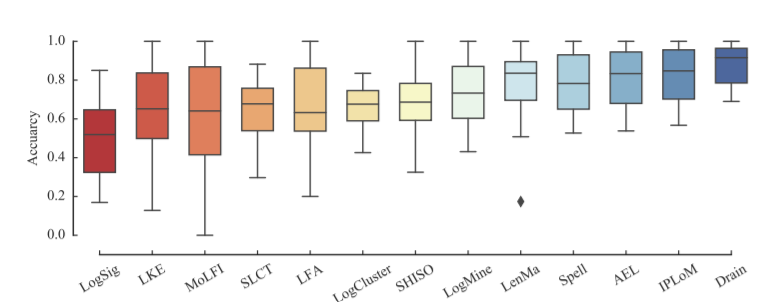
\includegraphics[width= \linewidth]{graph.png}
    \caption{Grafiek uit de paper `Tools and Benchmarks for Automated Log Parsing`~\autocite{TBA2019}}
\end{figure}

%---------- Verwachte conclusies ----------------------------------------------
\section{Verwachte conclusies}
\label{sec:verwachte_conclusies}

De nulhypothese van dit onderzoek is als volgt, op basis van literatuuronderzoek:\\
Drain zal naar boven komen als de meest geschikte log parser vanwege zijn efficiëntie en accuraatheid.

Het is de bedoeling om deze hypothese te confirmeren of te verwerpen en te zoeken naar een betere oplossing, dit zijnde een andere log parser, voor het parsen in een realtime setting omdat qua snelheid van parsing er nog altijd een grote beperking heerst zelfs met Drain.



%%---------- Andere bijlagen --------------------------------------------------
% TODO: Voeg hier eventuele andere bijlagen toe
%\input{...}

%%---------- Referentielijst --------------------------------------------------

\printbibliography[heading=bibintoc]

\end{document}
